\section{Results and Analysis}

In order to analyze the algorithms, we used both PAPI events and timed the algorithms for differently sized matrixes.
The data collected was saved in csv files and transformed into graphics for better analysis.

\subsection{PAPI events analysis}

The comparison of the \textbf{data cache misses} in L1 and L2 (PAPI\_L1\_DCM and PAPI\_L2\_DCM) between \textbf{Normal Matrix Multiplication} and \textbf{Multi-line Matrix Multiplication} draws us corroborate our theories: the second method of matrix multiplication avoids many cache misses. Although we expected to see a higher number of L1 cache misses than L2 cache misses, because there are some data that might not be present in L1 cache but might be present in L2 cache, our data contradicts this fact.

\begin{figure}[!h]
    \centering
    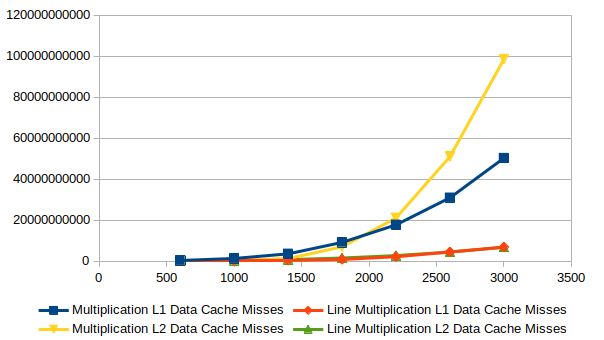
\includegraphics[width=.8\linewidth]{img/small_cache.png}
    \caption{Number of cache misses related to matrix size}
\end{figure}
